\section{Apepndix}
\begin{figure}[H]
    \centering
    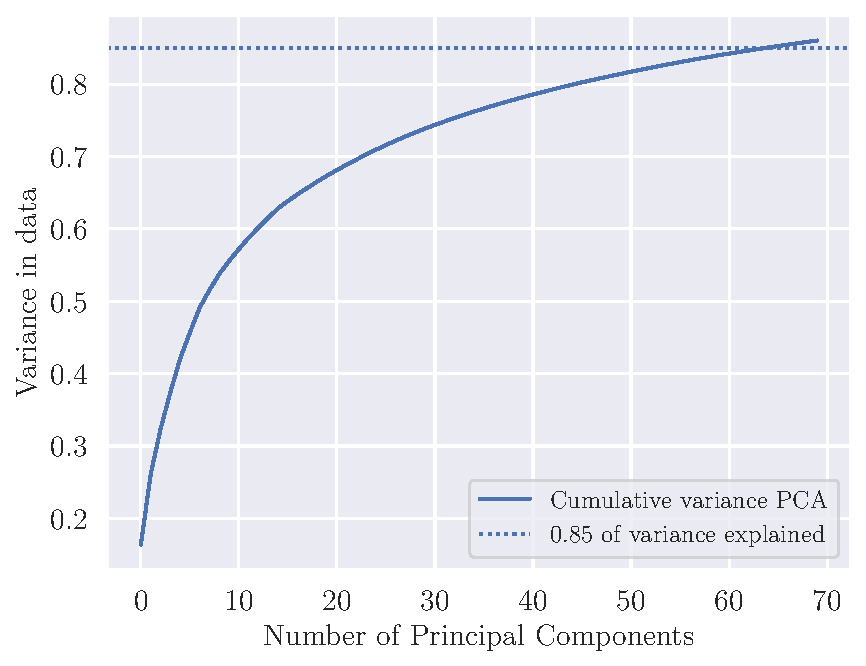
\includegraphics[width=0.9\linewidth]{examples/tests_eb/figs/cumsum_pca.pdf}
    \caption{A plot of the cumulative variance for each principle component included in our new, dimensionality reduced features. We concluded that 70 features was sufficient to capture just above 85 percent of the variance in our data.}
    \label{fig:cumsumpca}
\end{figure}

\begin{figure}[H]
    \centering
    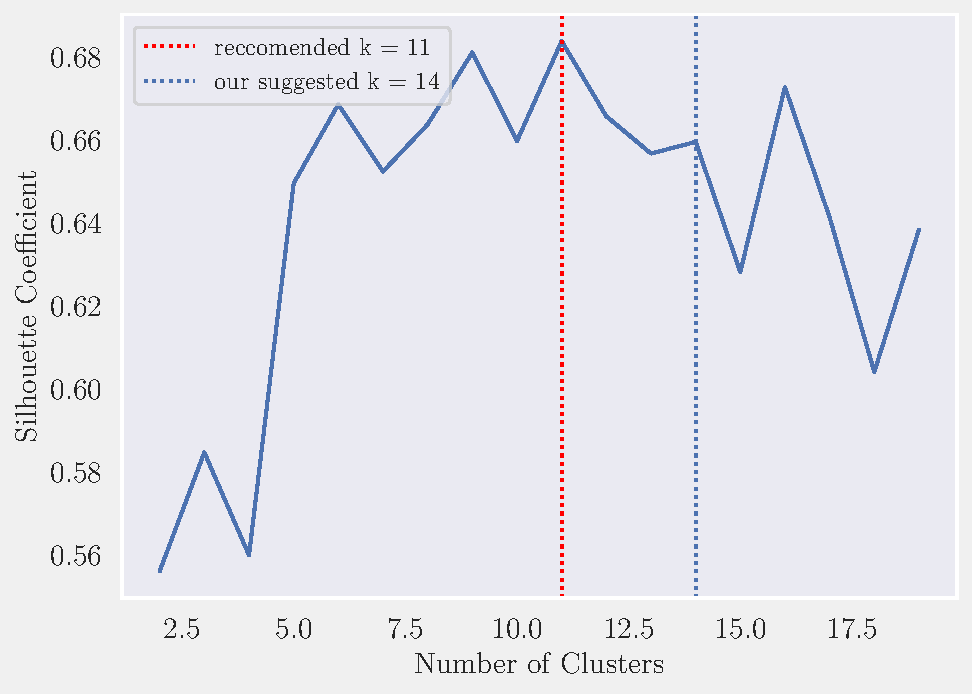
\includegraphics[width=0.9\linewidth]{examples/tests_eb/figs/kmean_sil.pdf}
    \caption{A plot of the silhouette scores for each KMean tested on UMAP data.}
    \label{fig_cumsumpca}
\end{figure}


\begin{figure}[H]
    \centering
    \begin{subfigure}[b]{1\linewidth}
        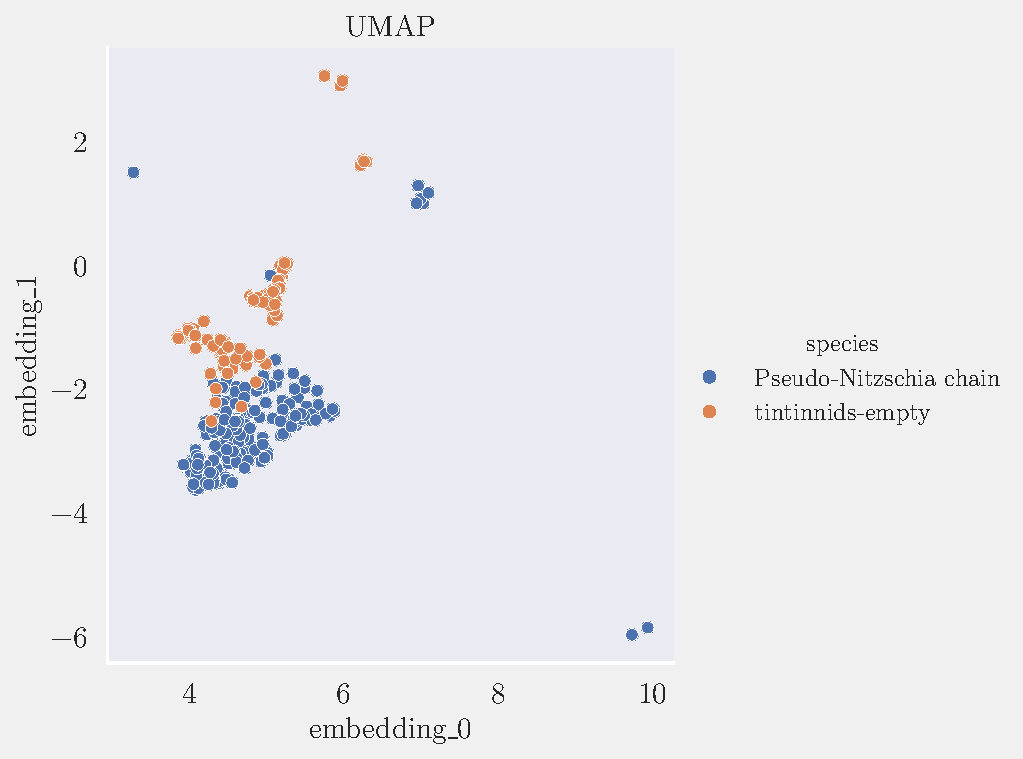
\includegraphics[width=\linewidth]{examples/tests_eb/figs/umap_on_two_species.pdf}
        \caption{First we isolated the already produced embeddings for the two species. Already her we can see that they form clysters according to their species.}
    \end{subfigure}
    
    \vspace{1em}
    
    \begin{subfigure}[b]{1\linewidth}
        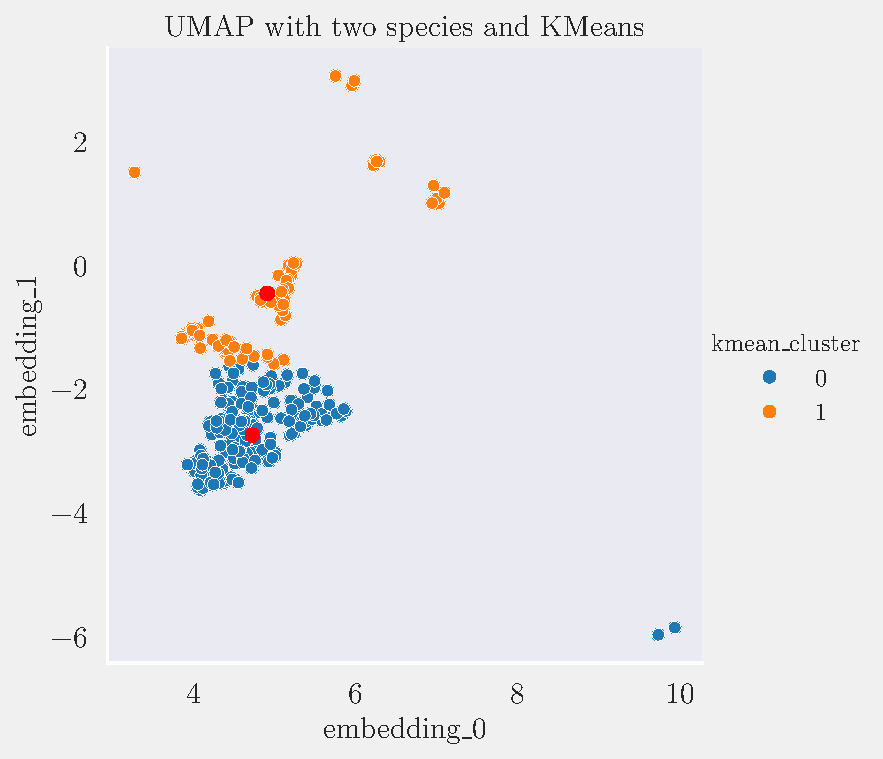
\includegraphics[width=\linewidth]{examples/tests_eb/figs/kmeans_cluster_umap_on_two_species.pdf}
        \caption{We performed a KMeans clustering with two clusters to find which images (or species) would cluster together in the embedding space. Red dots are kmer centroids.}
    \end{subfigure}
    \caption{The process of finding the images that misclusteded in Figure \ref{fig:misclusters} explained. We display images of Pseudo N that were placed in cluster 1, and the opposite for Tintinnids-e.}
    \label{fig:misclustering_process}
\end{figure}
